\documentclass[a4paper,12pt]{article}
\usepackage{a4wide}
\usepackage[pdftex]{hyperref}
\usepackage[german]{babel}
\usepackage[utf8]{inputenc}
\usepackage{amssymb}
\usepackage{csquotes}
\usepackage{wrapfig}
\usepackage{graphicx}
\usepackage{multicol}
\usepackage{amsmath}
\usepackage{enumitem}
\usepackage{polynom}
\usepackage{siunitx}

\setlength{\marginparsep}{1 cm}
\setlength{\topmargin}{-0.6in}
\setlength{\textheight}{9.5in}
\pagestyle{plain}

\polyset{%
   style=C,
   delims={\big(}{\big)},
   div=:
}

% Polynomial long division
\polyset{%
	style=C,
	delims={\big(}{\big)},
	div=:
}

% Differential operator
\newcommand{\diff}[1]{\:\mathrm{d}{#1}}
\newcommand{\pdd}[2]{\frac{\partial #1}{\partial #2}}
\newcommand{\pddn}[3]{\frac{\partial^{#1} #2}{\partial #3^{#1}}}
\newcommand{\dd}[2]{\frac{\mathrm{d}{#1}}{\mathrm{d}{#2}}}
\newcommand{\ddn}[3]{\frac{\mathrm{d}^{#1}{#2}}{\mathrm{d}{#3^{#1}}}}

% N-th root
% \nroot{3}{27}
\newcommand*{\nroot}[2]{\sqrt[\leftroot{-1}\uproot{2}#1]{#2}}
\newcommand*{\ncroot}[4]{\sqrt[\leftroot{#1}\uproot{#2}#3]{#4}}

% 2 component vector
% \tvect{1}{-1}
% \tvec{1}{-1}
\newcommand{\tvect}[2]{%
   \ensuremath{\Bigl(\negthinspace\begin{smallmatrix}#1\\#2\end{smallmatrix}\Bigr)}}
\newcommand{\tvec}[2]{%
    \ensuremath{\left(\negthinspace\begin{matrix}#1\\#2\end{matrix}\right)}}

% 3 component vector
% \rvect{1}{-1}{0}
% \rvec{1}{-1}{0}
\newcommand{\rvect}[3]{%
   \ensuremath{\Bigl(\negthinspace\begin{smallmatrix}#1\\#2\\#3\end{smallmatrix}\Bigr)}}
\newcommand{\rvec}[3]{%
    \ensuremath{\left(\negthinspace\begin{matrix}#1\\#2\\#3\end{matrix}\right)}}

% Long vector arrow
% \xshlongvec{ABC}

% German-style quotation marks %
\MakeOuterQuote{"}

% Number sets
\newcommand{\N}{\mathbb{N}}
\newcommand{\Z}{\mathbb{Z}}
\newcommand{\Q}{\mathbb{Q}}
\newcommand{\R}{\mathbb{R}}
\newcommand{\C}{\mathbb{C}}

\newcommand{\setzero}{\varnothing}

% Mention (small caps)
\newcommand{\mention}[1]{\textsc{#1}}

% Functions
\newcommand{\asin}[0]{\text{asin}}
\newcommand{\acos}[0]{\text{acos}}
\newcommand{\atan}[0]{\text{atan}}
\newcommand{\sgn}[0]{\text{sgn}}
\newcommand{\grad}[0]{\text{grad}}

% Scale
% Usage in math mode: \Scale[1.5]{...equation...} %
\newcommand*{\Scale}[2][4]{\scalebox{#1}{$#2$}}%

% Units
\newcommand{\um}{\text{m}}
\newcommand{\us}{\text{s}}
\newcommand{\ukm}{\text{km}}
\newcommand{\ukg}{\text{kg}}
\newcommand{\uh}{\text{h}}
\newcommand{\ukmh}{\frac{\ukm}{\uh}}
\newcommand{\umpers}{\frac{\um}{\us}}
\newcommand{\umss}{\frac{\ukm}{\us^2}}
\newcommand{\ukgss}{\frac{\ukg}{\us^2}}
\newcommand{\degrees}[1]{\SI{#1}{\degree}}

% Floor / ceil
\newcommand{\floor}[1]{\left\lfloor #1 \right\rfloor}
\newcommand{\ceil}[1]{\left\lceil #1 \right\rceil}

% Circle characters
\newcommand*\circled[1]{
    \tikz[baseline=(char.base)]{
        \node[shape=circle,draw,inner sep=2pt] (char) {#1};
    }
}



\begin{document}

\begin{center}
  {\bf {\large Aufgabenblatt 3 (MI/IT 2020)}}
\end{center}

% Tasks

\begin{enumerate}

\item Geben Sie irgendeine periodische Funktion an, deren Bildbereich gleich $[8,12]$ ist.


\item 
Gegeben ist die Funktion $f(x,y) = e^{x^2 / y}$.
Betrachten Sie deren Höhenlinie, die durch die Stelle $(x_0|y_0)=(1|2)$ läuft. Skizzieren Sie diese auf dem Bereich $[-2;2]\times[-2;2]$.
Wie sieht die Funktion zu den beiden Seiten der Höhenline hin aus, d.h. in welche Richtung zeigt der Gradient?



\item Der Definitionsbereich und der Wertebereich einer einstelligen Funktion sind jeweils Mengen, die aus reellen Zahlen bestehen. Aus welchen mathematischen Objekte besteht der Definitionsbereich und Wertebereich einer dreistelligen Funktion? Geben Sie den Definitionsbereich für $f(x,y,z) = \frac{y^z}{\ln(|x-2|)\sqrt{x+4})}$ an!

\item Leiten Sie folgende Funktion nach $x$ ab:
\begin{multicols}{3}
	\begin{enumerate}
	\item $f(x) = \sin((x+3)^2)$
	\item $g(x) = \sin(\sqrt x)$
	\item $h(x) = (e^x \ln(x))^3$
	\end{enumerate}
\end{multicols}

\item Ermitteln Sie von $y(x)=x^x$ die Ableitung! (Hinweis: Auf beide Seiten Logarithmus anwenden, per Kettenregel beide Seiten ableiten, nach $y'$ umstellen.)

\item An eine zunächst unbekannte Stelle $x_0$ des Graphen von $y=\frac{1}{x}$ wird die zugehörige
Tangentengerade gelegt. Man stellt fest, dass sie die $x$-Achse bei $x=7$ schneidet. Bestimmen
Sie $x_0$!


\item (*) Zeigen Sie anhand der Definition der Ableitung über den Differenzenquotienten, dass $\dd{}{x} e^x = e^x$ gilt! Hinweis: Substitution $z=e^\varepsilon-1$ und nutzen Sie die Übersicht über Grenzwerte einiger spezieller konvergenter Folgen aus der Vorlesung.


\item Bestimmen Sie für $f(x,y) = x^2 + 4xy -2y^2$ die Gleichung der Tangentialebene an der Stelle $(2,1)$! [Zusatz Vektorrechnung]: Geben Sie weiterhin die Tangentialebene in Hessescher Normalform und parametrischer Form an!


\item
$f(u,v,w) = \frac{u^2 \sin(3v) +4}{w}$.
Leiten Sie f partiell nach u, nach v und nach w ab, d.h. bestimmen Sie $\frac{\partial^2 f}{\partial u \partial v}(u,v,w)$, $\frac{\partial^2 f}{\partial v \partial u}(u,v,w)$ sowie $\frac{\partial^2 f}{\partial w^2}(u,v,w)$! Stimmt bei diesem Beispiel der Satz von Schwarz?



\item Ein Körper ruht auf einer Gummimatte an der Stelle $s=0$. Zur Zeit $t=0$ wird er nach oben geworfen. Kurze Zeit später landet er wieder auf der Gummimatte, wobei der Körper leicht nach unten in die Gummimatte sinkt, welche sich anschließend wieder ausdehnt und den Gegenstand zurück in die Höhe $s=0$ der Gummimatte bringt. Dabei ist $s$ die Höhe über der Gummimatte.  Die Orts-Zeit-Kurve für diesen Vorgang laute $s(t) = t^3-15t^2+54t$. Berechnen Sie den Zeitpunkt $t_1$, zu dem der Körper landet und den Zeitpunkt $t_2$, an dem der Körper wieder in Höhe $s=0$ zurückgekehrt ist! Ermitteln Sie ferner eine Formel für die Geschwindigkeit $v(t) = \dd{}{t}s(t)$ und die Beschleunigung $a(t) = \ddn{2}{}{t}s(t)$! Wie groß ist die Minimal- und Maximalgeschwindigkeit des Körpers im Zeitraum $[0,t_2]$? Berechnen Sie schließlich die Durchschnittsgeschwindigkeit des Körpers im Zeitraum $[0,t_1]$. Hinweis: Die Durchschnittsgeschwindigkeit in einem Zeitraum $[t',t'']$ ist gegeben durch $\bar{v} = \frac{1}{t''-t'}\int\limits_{t'}^{t''} |v(t)| \diff{t}$

\end{enumerate}

\newpage

% Solutions

\begin{center}
{\bf {\large Lösungen}}
\end{center}

\begin{enumerate}
	
\item  Der Bildbereich ist nach unten und nach oben beschränkt, es bietet sich also eine modifizierte trigonometrische Funktion an:

Zum Beispiel: $f(x) = 2\sin(x) +10$ oder $g(x) = 2\cos(x) +10$



\item 

Die Höhenlinie ist die Menge aller Punkte $(x,y)$, wo die Funktion den gleichen Funktionswert besitzt, $f(x,y) = const.$ Zur Bestimmung dieser Konstanten setzen wir den Punkt $(x_0,y_0)$ ein:

$f(x,y) = f(1,2)$

$\implies e^{\frac{x^2}{y}} = e^{\frac{1}{2}}$

$\implies \frac{x^2}{y} = \frac{1}{2}$

$\implies y = 2x^2$

Die gesuchte Höhenlinie ist also eine Parabel, die um den Faktor $2$ entlang der y-Achse gestreckt ist.

Zur Bestimmung des Gradienten benötigen wir die partiellen Ableitung nach x und y:

$\frac{\partial f}{\partial x} =  \frac{2x}{y} \cdot e^{\frac{x^2}{y}}$

$\frac{\partial f}{\partial y} =  e^{\frac{x^2}{y}} \cdot (-y^{-2} \cdot x^2) = - \frac{x^2}{y^2} \cdot e^{\frac{x^2}{y}} $

Einsetzen der Höhenlinie $y=2x^2$:

$\frac{\partial f}{\partial x}|_{y=2x^2}=  e^{\frac{x^2}{2x^2}} \cdot \frac{2x}{2x^2} = e^{\frac{1}{2}}\cdot \frac{1}{x}$

$\frac{\partial f}{\partial y}|_{y=2x^2} =  -e^{\frac{x^2}{2x^2}} \cdot \frac{x^2}{4x^4} = -e^{\frac{1}{2}}\cdot \frac{1}{4x^2}$

Der Gradient auf der Höhenlinie zeigt immer in negative y-Achenrichtung (nach unten).

In der rechten Halbebene zeigt er in positive x-Richtung (nach rechts), in der linken Halbebene in negative x-Richtung (nach links).

\begin{figure}[ht]
\centering
  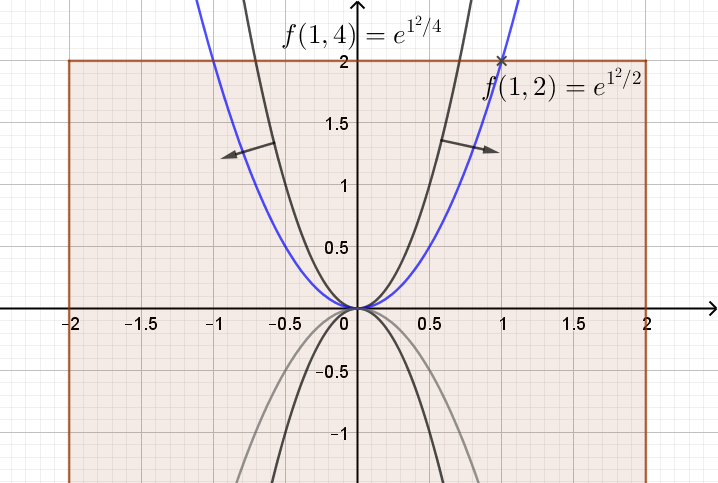
\includegraphics[width=0.4\textwidth]{../pool/ex-graph-contour-1-img-a.png}
  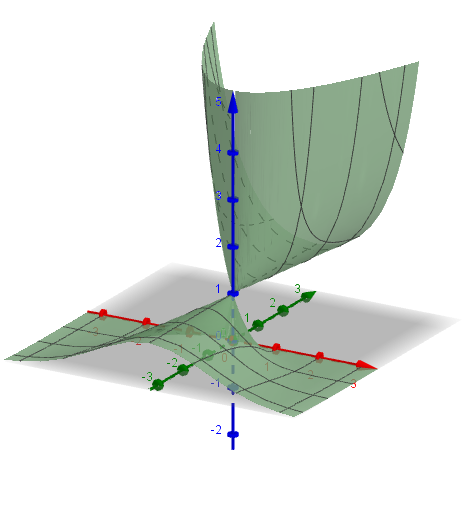
\includegraphics[width=0.4\textwidth]{../pool/ex-graph-contour-1-img-b.png}
  \caption{Höhenlinie mit Gradient zur Höhenlinie $f(x,y)=f(1,2)$ (links) und 3D-Plot davon (rechts)}
\end{figure}



\item Der Definitionsbereich einer dreistelligen Funktion besteht aus 3-Tupeln von reellen Zahlen, welche ein kartesisches Produkt darstellen: $\R\times\R\times\R=\R^3$. Der Wertebereich besteht wie bei einstelligen Funktionen aus reellen Zahlen.

Wir betrachten die Funktion

$$
	f(x,y,z) = \frac{y^z}{\ln(|x-2|)\sqrt{x+4})}
$$

Folgende Einschränkungen gelten:

\begin{itemize}
	\item Das Argument des Logarithmus muss positiv sein, also $x\ne 2$
	\item Das Argument der Wurzel darf nicht negativ sein, also $x \ge -4$
	\item Der Nenner darf nicht identisch $0$ sein. Damit darf das Argument des Logarithmus nicht 1 sein (da $\ln(1) = 0$), also $x \ne 3$ und $x \ne 1$. Andererseits darf auch das Argument der Wurzel nicht $0$ sein, also $x > -4$.
	\item Der Ausdruck $0^0$ ist nicht definiert, daher dürfen $y$ und $z$ nicht beide gleichzeitig identisch $0$ sein.
\end{itemize}

Zusammengefasst erhalten wir also folgenden Definitionsbereich:

$$
	\mathbb{D} = \lbrace (x,y,z) \in \R^3 \hskip 2mm | \hskip 2mm  [x \in (-4,\infty) \setminus \lbrace 1,2,3 \rbrace ] \land [ y \ne 0 \lor z \ne 0 ] \rbrace
$$

\item
\begin{enumerate}

\item $\dd{}{x} \lbrack \sin((x+3)^2) \rbrack = 2(x+3)\cos((x+3)^2)$

\item

$\dd{}{x} \lbrack \sin(\sqrt x) \rbrack$

$=\frac{1}{2}(\cos(\sqrt x)x^{-\frac{1}{2}}$

$=\frac{1}{2\sqrt{x}}(\cos(\sqrt x)$

\item

$\dd{}{x} \lbrack (e^x \ln(x))^3 \rbrack $

$\stackrel{\text{Kettenregel}}{=} 3(e^x\ln(x))^2 \cdot \dd{}{x}[e^x\ln(x)]$

$\stackrel{\text{Produktregel}}{=} 3e^{2x}(\ln(x))^2(e^x\ln(x)+\frac{e^x}{x})$

$\stackrel{\text{ausklammern}}{=} 3e^{3x}(\ln(x))^2(\ln(x)+\frac{1}{x})$
\end{enumerate}



\item Wir gehen vor wie beschrieben:

\begin{alignat*}{1}
	y(x) &= x^x \\
	\ln(y(x)) &= \ln(x^x) = x\ln(x) \\
	\dd{}{x} \ln(y(x)) &= \dd{}{x} x\ln(x)
\end{alignat*}

Die rechte Seite kann normal per Produktregel abgeleitet werden. Auf der linken Seite müssen wir aufpassen, dass $y(x)$ eine Funktion von $x$ ist. Die äußere Ableitung bei der Kettenregel lautet $\frac{1}{y}$, die innere Ableitung $y'(x)$, insgesamt gilt also $\dd{}{x} \ln(y(x)) = \frac{y'}{y}$. Damit erhalten wir:

\begin{alignat*}{1}
	\frac{y'(x)}{y(x)} = \ln(x)+1 \\
	y'(x) = y(x)\cdot(\ln(x+1)) \\
	y'(x) = x^x \cdot (\ln(x)+1)
\end{alignat*}

Anmerkung: Die Weise des Ableitens nennt sich auch "logarithmisches Differenzieren". Auf die gleiche Weise lässt sich zeigen, dass allgemein die Ableitung von $f(x)^{g(x)}$, wobei $f,g$ zwei beliebige Funktionen sind, lautet:

$$
	\dd{}{x} f^g = f^g \cdot \left( g'\ln(f) + f' \frac{g}{f} \right)
$$

Aus dieser allgemeinen Regel lässt sich etwa mit $f=x, g=n$ die Ableitungsregeln für Monome gewinnen: $\dd{}{x}x^n = x^n(0+1\cdot\frac{n}{x}) = nx^{n-1}$. Für $f=a, g=x$ folgt die Regeln zum Ableiten von Exponentialfunktionen: $\dd{}{x} a^x = a^x (1\cdot\ln(a) + 0) = \ln(a)a^x$.

\item

Wir berechnen die Gleichung der Tangentengerade in Abhängigkeit vom Anlagepunkt $x_0$.

Der Anstieg $m$ der Tangenten folgt aus der 1. Ableitung:

$f'(x) = -\frac{1}{x^2}$

$\implies f'(x_0) = -\frac{1}{x_0^2}$

Der Funktionswert an der Stelle $x_0$ ergibt sich zu $f(x_0) = \frac{1}{x_0}$. Die Tangentengleichung $t(x)$ lautet somit:

$t(x) = f(x_0) + f'(x_0) (x-x_0) = \frac{1}{x_0} -\frac{1}{x_0^2} (x-x_0)$

Die Tangente schneidet die x-Achse in der Nullstelle $x_z$:

$t(x_z) = 0 = \frac{1}{x_0} -\frac{1}{x_0^2} (x_z-x_0)$

$\implies \frac{1}{x_0} = \frac{1}{x_0^2} (x_z-x_0) $

$\implies x_0 = x_z-x_0 $

$\implies x_z = 2x_0 $

Nach Aufgabestellung soll der Schnittpunkt der Tangente mit der x-Achse bei $7$ liegen, also $x_z = 2x_0 = 7$, somit $x_0 = 3.5$.



\item Per Definition gilt für Ableitung:

\begin{alignat*}{1}
	\dd{}{x}e^x &= \lim\limits_{\varepsilon\to 0} \frac{e^{x+\varepsilon}-e^x}{\varepsilon}\\
	            &= \lim\limits_{\varepsilon\to 0} e^x \frac{e^\varepsilon -1}{\varepsilon}
\end{alignat*}

Für ein gegebenes $x$ ist $e^x$ eine Konstante und kann vor die Grenzwertbildung gezogen werden. Um den verbleibenden Grenzwert zu berechnen, substituieren wir:

\begin{alignat*}{1}
	z &= e^\varepsilon - 1 \\
	\varepsilon &= \ln(z+1)
\end{alignat*}

Für $\varepsilon \to 0$ gilt ebenfalls $z \to 0$. Jetzt müssen wir folgenden Grenzwert berechnen:

\begin{alignat*}{1}
	  & \lim\limits_{z\to 0} \frac{z}{\ln(z+1)} \\
	= & \lim\limits_{z\to 0} \frac{1/\frac{1}{z}}{\ln(z+1)} \\
	= & \lim\limits_{z\to 0} \frac{1}{\frac{1}{z}\ln(z+1)} \\
	= & \lim\limits_{z\to 0} \frac{1}{\ln([z+1]^\frac{1}{z})} \\
	= & \frac{1}{\ln(\lim\limits_{z\to 0}[z+1]^\frac{1}{z})}
\end{alignat*}

Der letzte Schritt ist richtig, da nach den Grenzwertregeln für stetige Funktion die Grenzwertbildung und die Funktionsanwendung vertauscht werden können.

Statt den Grenzwert für $z\to 0$ auszuwerten, können wir auch $n=\frac{1}{z}$ setzen und stattdessen den Grenzwert $n\to\infty$ auswerten:

\begin{alignat*}{1}
	    \lim\limits_{z\to 0}[z+1]^\frac{1}{z} \\
	= & \lim\limits_{n \to \infty}[1+\frac{1}{n}]^n \\
	= & e
\end{alignat*}
	
Im letzten Schritt haben wir dabei von dem entsprechenden Grundgrenzwert Gebrauch gemacht (welchen man auch als Definition der Zahl $e$ verstehen kann). Damit ergibt sich  zusammengefasst für die Ableitung der Exponentialfunktion:

\begin{alignat*}{1}
	\dd{}{x}e^x &= e^x \cdot \lim\limits_{\varepsilon\to 0} \frac{e^\varepsilon -1}{\varepsilon} \\ 
	            &= e^x \cdot \frac{1}{\ln(\lim\limits_{z\to 0}[z+1]^\frac{1}{z})} \\
	            &= e^x \cdot \frac{1}{\ln(e)} \\
	            &= e^x \cdot \frac{1}{1} \\
	            &= e^x
\end{alignat*}
	
Dies war zu zeigen.


\item Funktionswert an der gegebenen Stelle: $f(2,1) = 4+8-2=10$. Nun zuerst ableiten:

\begin{itemize}
\item $f_x = 2x+4y$
\item $f_y = 4x-4y$
\end{itemize}

Nun an der Stelle $(2,1)$ auswerten:

\begin{itemize}
\item $f_x(2,1) = 4+4 = 8$
\item $f_y(2,1) = 8-4 = 4$
\end{itemize}

Damit ergibt sich für die Tangentialebene:

$$z = t(x,y) = 10 + 8(x-2) + 4(y-1)$$

\begin{itemize}
\item Hessesche Normalform: Ausklammern obiger Gleichung liefert $8x+4y-z=10$. Dies lässt sich schreiben als $\vec{n}\cdot\vec{x} = \rvect{8}{4}{-1}\cdot\rvect{x}{y}{z} = 10$. Der Normalvektor hat den Betrag $|\vec{n}| = \sqrt{8^2+4^2+1^2} = \sqrt{81} = 9$. Damit lässt sich sich Ebenengleichung umformen zu $\vec{n_0}\cdot\vec{x} = \rvect{8/9}{4/9}{-1/9}\cdot\rvect{x}{y}{z} = \frac{10}{9}$. Dies ist die Hessesche Normalform.
\item Parametrische Form: Diese liest man direkt aus der partiellen Ableitung ab: $\vec{r}(u,v) = \rvect{2}{1}{10} + u \cdot \rvect{1}{0}{8} + v \cdot \rvect{0}{1}{4}$
\end{itemize}



\item

$\frac{\partial f}{\partial u} = \frac{2u\sin(3v)}{w}$

$\frac{\partial f}{\partial v} = \frac{3u^2\cos(3v)}{w}$

$\frac{\partial^2 f}{\partial u \partial v} = \frac{\partial^2 f}{\partial v \partial u} = \frac{6u \cos(3v)}{w}$

$\frac{\partial^2 f}{\partial w^2} = (u^2\sin(3v)+4)\cdot \frac{2}{w^3}$

Bei richtiger Rechnung ergibt sich $\frac{\partial^2 f}{\partial u \partial v} = \frac{\partial^2 f}{\partial v \partial u}$, es liegt also kein Widerspruch zum Satz von Schwarz vor. 



\item Für die Zeitpunkte $t_1,t_2$ gilt, dass dort $s=0$ sein muss. Wir suchen also die Nullstellen von $0=t^3-15t^2+54t$. Da kein konstanter Faktor vorkommt, lautet eine Nullstelle $t_0=0$, dies ist der Abwurfzeitpunkt. Wir können faktorisieren $0=t^3-15t^2+54t=t \cdot (t^2-15t+54)$. Der zweite Faktor ist eine quadratische Gleichung:

$$
	t_{1,2} = \frac{15}{2} \pm \sqrt{\frac{15^2}{2^2} - 54} = \frac{15}{2} \pm \sqrt{\frac{225}{4} - \frac{216}{4}} = \frac{15}{2} \pm  \sqrt{\frac{9}{4}} = \frac{15}{2} \pm \frac{3}{2}
$$

Wir erhalten also $t_1 = 6$ und $t_2 = 9$.

Als nächstes leiten wir ab:

\begin{alignat*}{1}
	s(t) &= t^3-15t^2+54t \\
	v(t) &= 3t^2-30t+54 \\
	a(t)&= 6t-30
\end{alignat*}

Die Maximal- und Minimalgeschwindigkeit erhalten wir, in dem wir die Extremstellen der Geschwindigkeit $v$ betrachten. Für lokale Extremstellen muss $\dd{}{t}v=a=0$ gelten, also $6t-30=0$. Wir erhalten als Kandidat $t=5$. Da es sich bei $v$ um eine nach oben geöffnete Parabel handelt, liegt bei $t=0$ ein lokales Minima vor (was wir auch bestätigen könnten durch die dritte Ableitung: $a'(t)=6>0$). Die Geschwindigkeit zu diesem Zeitpunkt beträgt $v(5)=3\cdot 25-30\cdot 5+54=75-150+54=-21$ Zudem kann es aber auch noch globale Extremstellen geben. Dazu müssen wir die Grenzen des betrachteten Zeitraums betrachten. Für $t_0=0$ erhalten wir $v(0)=54$, für $t_2=9$ ergibt sich $v(9)=3\cdot 81-30\cdot 9+54 = 3\cdot(81-3\cdot 30)+54 = 3\cdot (-9) + 54 = 27$.

Also lautet die Minimalgeschwindigkeit $v(5)=-21$, die Maximalgeschwindigkeit $v(0)=54$.

Für die Durchschnittsgeschwindigkeit im Zeitraum $[0,6]$ müssen wir über den Betrag der Geschwindigkeit teilen. Dazu teilen wir das Integrationsintervall an der Nullstelle. Die Nullstellen von $v(t)=3t^2-30t+54$ lauten:

\begin{alignat*}{1}
	0 &= t^2-10t+18 \\
	t &= 5 \pm \sqrt{25-18} = 5 \pm \sqrt{7}
\end{alignat*}

Es kommt nur die Lösung $5 - \sqrt{7}$ in Betracht, da die andere Lösung außerhalb des betrachteten Intervalls liegt.

Die Durchschnittsgeschwindigkeit berechnet sich nun -- unter Beachtung der Tatsache, dass $s$ eine Stammfunktion von $v$ ist und dass die Geschwindigkeit $v$ links der Nullstelle positiv und rechts davon negativ ist -- zu:

\begin{alignat*}{1}
	\bar{v} &= \frac{1}{6} \left( \int\limits_0^6 |v(t)| \diff{t} \right) \\
	        &= \frac{1}{6} \left( \int\limits_0^{5-\sqrt{7}} v(t) \diff{t} - \int\limits_{5-\sqrt{7}}^6 v(t) \diff{t} \right) \\
	        &= \frac{1}{6} \left( s(5-\sqrt{7}) -s(0) - s(6) + s(5-\sqrt{7}) \right) \\
	        &= \frac{s(5-\sqrt{7})}{3}
\end{alignat*}

Im letzten Schritt haben wir davon Gebrauch gemacht, dass $s(0)=s(6)=0$ gilt, da es sich um die Nullstellen von $s$ handelt. Es verbleibt, $s(5-\sqrt{7})$ zu berechnen:

\begin{alignat*}{1}
	s(5-\sqrt{7}) &= (5-\sqrt{7})^3 -15 (5-\sqrt{7})^2+54(5-\sqrt{7}) \\
	              &= (230-82\sqrt{7}) -15(32-10\sqrt{7})+54(5-\sqrt{7}) \\
	              &= 230-82\sqrt{7}-480+150\sqrt{7}+270-54\sqrt{7} \\
	              &= 20+14\sqrt{7}
\end{alignat*}

Damit erhalten wir für die Durchschnittsgeschwindigkeit:

$$
	\bar{v} = \frac{20+14\sqrt{7}}{3}
$$



\end{enumerate}

\end{document}

